
\documentclass[twocolumn]{aastex62}

\newcommand{\vdag}{(v)^\dagger}
\newcommand\aastex{AAS\TeX}
\newcommand\latex{La\TeX}

\graphicspath{{./}{figures/}}


\submitjournal{ApJ}

\shorttitle{Radiation Feedback in Dwarf Galaxies}
\shortauthors{Emerick et. al.}


\begin{document}

\title{Stellar Radiation is Critical for Regulating Star Formation and Driving Outflows in Low Mass Dwarf Galaxies}

\correspondingauthor{Andrew Emerick}
\email{emerick@astro.columbia.edu}

\author{Andrew Emerick}
\affil{Columbia University}
\affil{American Museum of Natural History (AMNH)}

\author{Greg L. Bryan}
\affiliation{Columbia University}
\affiliation{Flatiron Institute}

\author{Mordecai-Mark Mac Low}
\affiliation{American Museum of Natural History (AMNH)}
\nocollaboration

\begin{abstract}
Ionizing radiation from recently formed massive stars is important in destroying cold, dense gas around new regions of star formation that would otherwise continue to form stars. Applying a local prescription for this pre-supernova feedback can be sufficient in matching star formation rates in a simulation with full radiative transfer on short timescales. However, the long-range effects of ionizing radiation are important in producing a volume-filling diffuse, warm-ionized medium in the ISM and in the disk-halo interface. This is essential for allowing supernovae to drive significant gas outflows that travel throughout and beyond the virial radius of the galaxy. A simulation with local radiation feedback only is unable to drive significant outflows as the supernovae are trapped well within the inner halo by higher density cold and warm neutral gas.
\end{abstract}

%% Keywords should appear after the \end{abstract} command. 
%% See the online documentation for the full list of available subject
%% keywords and the rules for their use.
\keywords{galaxies -- feedback -- galaxy evolution -- galactic winds}

\section{Introduction} \label{sec:intro}
Overview of importance of pre-SN feedback in regulating SF. Brief literature overview of recent simulations with full radiative transfer. Brief mention / discussion of current approximations / simplifications made in runs without RT that include something for radiation feedback. Motivate how it is unclear as to whether or not full fancy RT physics is necessary, or if 1) can just do SNe (unlikely), and 2) can just get by with local (e.g. Stromgren) approximation. How might this affect global galaxy properties beyond SFR?

Key here is that radiation affects role of SNe in driving galactic winds. This is known already (Peters2016, Hu2016, Hu2017, and more), but has not been demonstrated like this for outflowing properties, primarily b/c many methods use approximate effects of RT. 

\section{Methods and Initial Conditions} \label{sec:methods}
We refer the reader to Paper I for a more detailed description of our methods, briefly summarized here. We use the adaptive mesh refinement hydrodynamics code \textsc{Enzo} \citep{Enzo} to evolve an idealized, isolated low mass dwarf galaxy initialized as a smooth exponential disk set in hydrostatic equillibrium with a static dark matter potential with $M_{\rm gas} = 2 \times 10^6~$~M$_{\odot}$, radial and vertical gas scale heights of 250~pc and 100~pc respectively, $M_{\rm vir} = 2.48 \times 10^9$~M$_{\odot}$, and a maximum physical resolution of 1.8~pc. We include a UV background, tabulated metal line cooling, and a 9 species non-equillibrium chemistry solver using \textsc{Grackle} \citep{Grackle}. Star formation occurs stochastically in cold, dense regions ($n > 200$~cm$^{-3}$, $T < 200$~K) by sampling the \cite{Salpeter1995} IMF from 1~M$_{\odot}$ to 100~M$_{\odot}$ and depositing \textit{individual} star particles over this mass range. For each star, we include feedback from stellar winds, AGB winds, FUV and LW band radiation which drives photoelectric heating and H$_2$ dissociation respectively, HI and HeI ionizing radiation, and core collapse and Type Ia SNe using thermal energy injection. FUV and LW band radiation are both taken to be optically thin, which approximate, local self-shielding alone, but ionizing radiation is followed with radiative transfer (see below). 

\textbf{Stellar Ionizing Radiation Models} $-$ We present a comparison of three simulations in this work, which are identical with the exception of their stellar ionizing radiation feedback. In our fiducial simulation, we track the HI and HeI photoionizing radiation using the adaptive ray-tracing radiative transfer method of \citep{MORAY} for all stars above 8$M_{\odot}$ (see Paper I for details on determining the ionizing photon rates for each star). We additionally present a simulation run without any stellar ionizing radiation (``noRT'') and a second simulation to test the relative importance of short-range vs. long-range effects of the radiation where we follow the full ionizing radiation RT, but delete photons once they have traveled more than 20~pc from their source (``shortrad''). This last simulation performs a similar, though significantly more detailed, function as commonly used methods to account for stellar radiation feedback which either deposit thermal energy (citation) or thermal energy and ionization (citations) locally, typically within the Stromgren radius, of each star.  Each simulation is identical up until the formation of the first star particles, at which point they begin to diverge. We note that the stars from the very first star formation event in each run (21 star particles with a total mass of 114 M$_{\odot}$) are the same in each run. Of these, one particle emits ionizing radiation ($M_* > 8 $~M$_{\odot}$). 

\section{Results} \label{sec:results}

\begin{figure*}
\centering
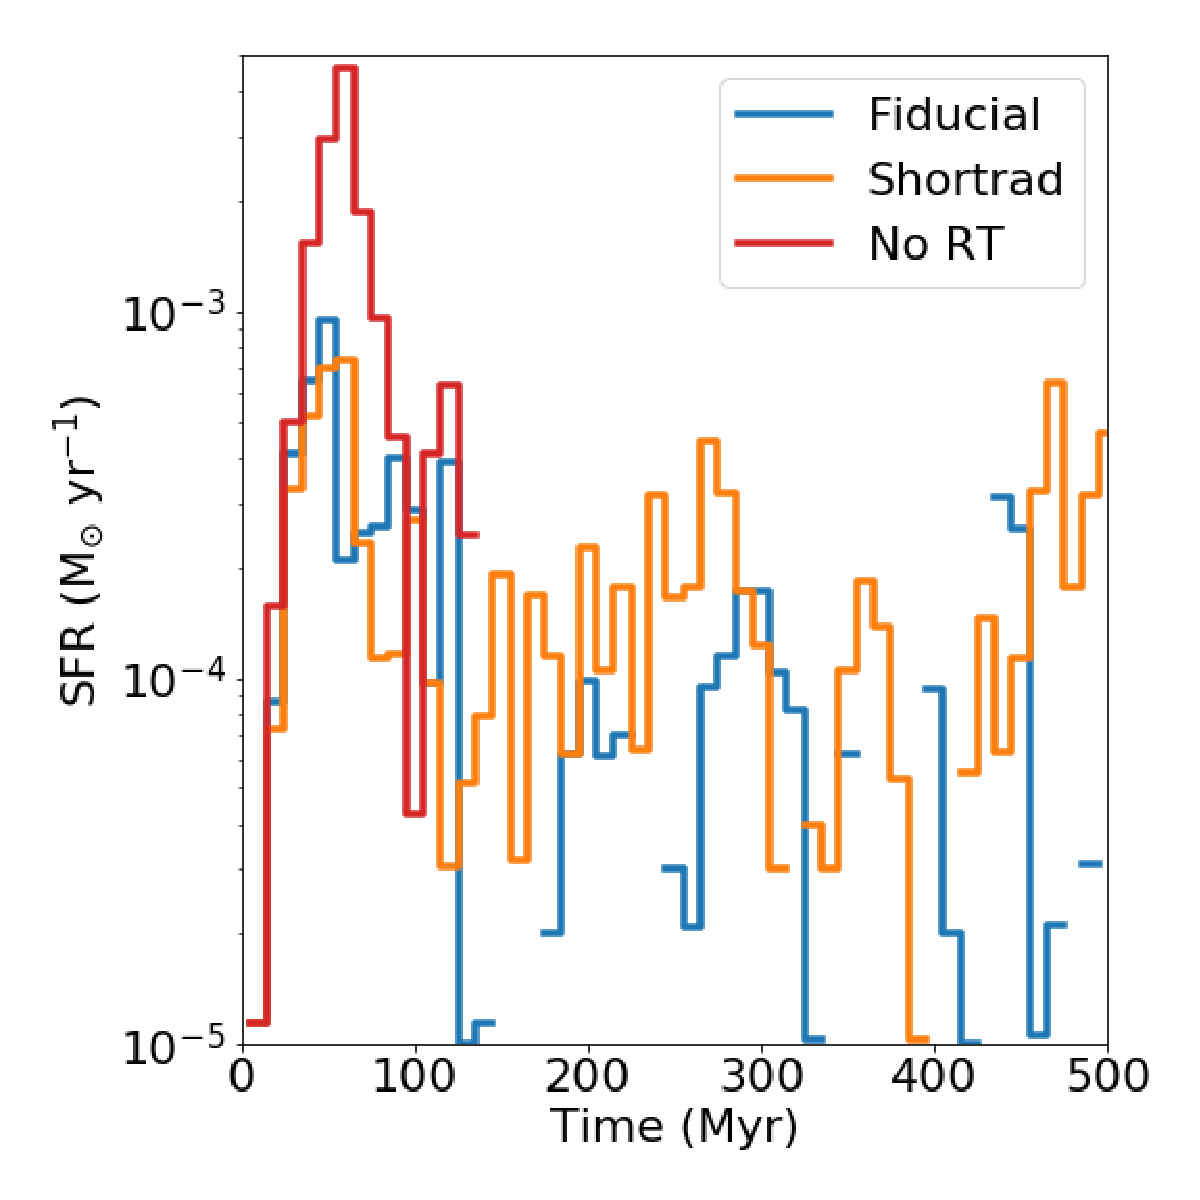
\includegraphics[width=0.49\linewidth]{sfr}
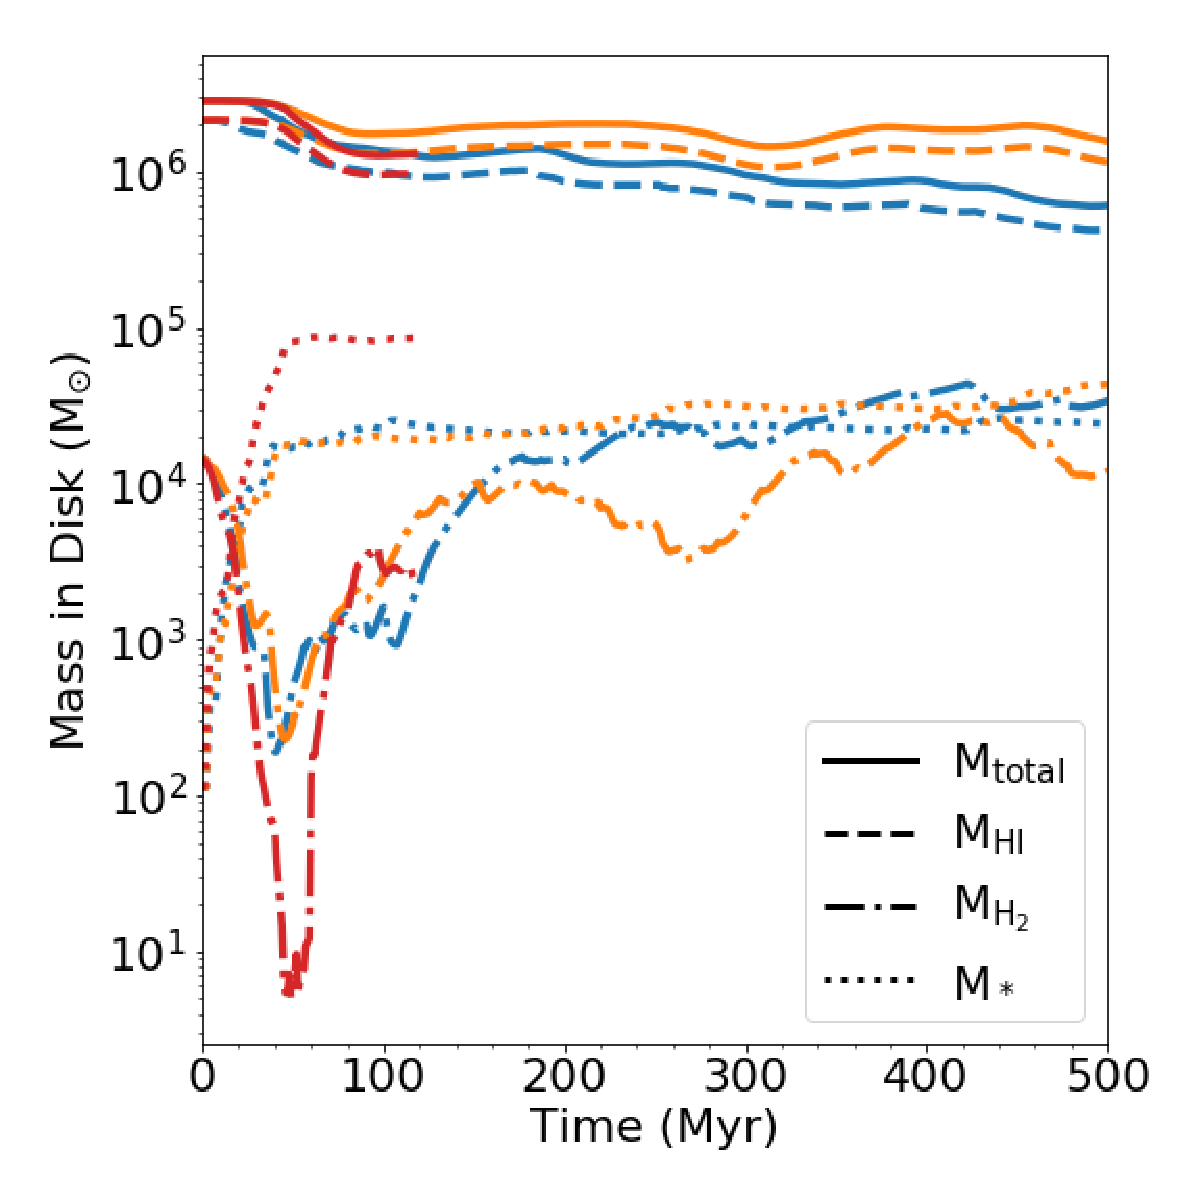
\includegraphics[width=0.49\linewidth]{mass}
\caption{}
\label{fig:sfr_mass_evolution}
\end{figure*}

We compare the resulting star formation rate (left) and gas mass properties (right) of our three simulations in Figure~\ref{fig:sfr_mass_evolution}. There is a clear, significant contrast between the runs with and without ionizing radiation. Stellar ionizing radiation leads to a factor of $\sim$ 5 reduction in the resulting SFR, as compared to the noRT run. Since the shortrad and fiducial simulations are so similar over the first $\sim$~100~Myr, it is clear that stellar radiation acts to significantly reduce the local star formation efficiency around young, massive stars. Radiation from these stars quickly ionizes and dissipates surrounding dense gas that would otherwise have gone to fuel a significant amount of additional star formation. We are unable to follow the long-term evolution of the noRT galaxy due to computational constraints. Although radiative transfer is expensive, this run is substantially more computationally expensive than the fiducial and shortrad runs due to the significantly higher star formation rate.

Looking again at the first $\sim$100~Myr of simulation time, the effects of ionizing radiation beyond our 20~pc cutoff radius are not significant. However, these two simulations begin to diverge significantly after this point. The shortrad simulations has continual, steady star formation for the entire simulation time, while the star formation rate in our fiducial run is bursty, with periods of active, low-level star formation interspersed with periods (sometimes up to 50~Myr) of no star formation. The driver of these differences is clear in the right hand panel. Our fiducial run looses a significant amount of total gas and HI mass (black and blue lines) as compared to the shortrad simulation by a factor of XX. Clearly, galactic winds and outflows are much more effective in the fiducial case, with full accounting of stellar ionizing radiation feedback, then in the shortrad simulation.

This can be confirmed by examining the mass loading factor and metal retention fraction (the fraction of produced metals retained within the disk of the galaxy) in each simulation. As shown in Figure~\ref{fig:metal_retention}, the mass loading factor in the fiducial run is a factor of XXX higher at 0.25~R$_{\rm vir}$ than the shortrad simulation, and is the only simulation with any significant outflow beyond the virial radius. This is especially interesting considering the factor 5 increase in SFR of the noRT run. The noRT run does have a significant amount of gas mass outflowing at XXXX, but note that its low mass loading factor is due primarily to the significantly larger SFR in this galaxy. Radiation feedback, both locally and over longer ranges, is important in determining the ability for SN to drive significant outflows. We discuss the reasons for this in the following section.

\section{Discussion} \label{sec:discussion}
Again, it is known that accounting for feedback from stellar radiation plays a significant role in determining the ability for SN energy to couple to the ISM and therefore drive outflows. However, the specific importance of localized ionization vs. ionization far from the source star has not been examined. As shown above, accounting for stellar radiation feedback locally alone is insufficient to describe the long-term evolution of an isolated dwarf galaxy. To explore the cause of this difference we present two panel-plots in Figure~\ref{fig:panel1} and Figure~\ref{fig:panel2} which compare the gas number density (left), temperature (middle), and HI ionization fraction (right) in edge-on slices in each of our simulations at two different times.\footnote:{See ({\it insert link here}) for a movie of this comparison} 

Figure~\ref{fig:panel1}, at XX Myr, shows each just after the first few SN in each simulation. Already there are significant differences across runs. Gas outside the galaxy is warm ($\sim$~10$^{4}$~K) and ionized up to XX~pc above/below the plane of the disk in our fiducial run. This same gas is cold ($<10^4$~K) and neutral in both other runs. The contrast between the fiducial and shortrad radiation is seen most clearly in the ionized region in-plane and to the right of center in the top and bottom panels. This region contains massive stars that are capable of generating enough ionizing radiation to carve a channel out to the halo of our fiducial simulation; by construction, this does not occur in the shortrad case. The warm / ionized feature towards the center of each galaxy is gas from a recent SN. This is much more well contained and hotter in the noRT and shortrad runs than in our fiducial simulation. 

\begin{figure*}
\centering
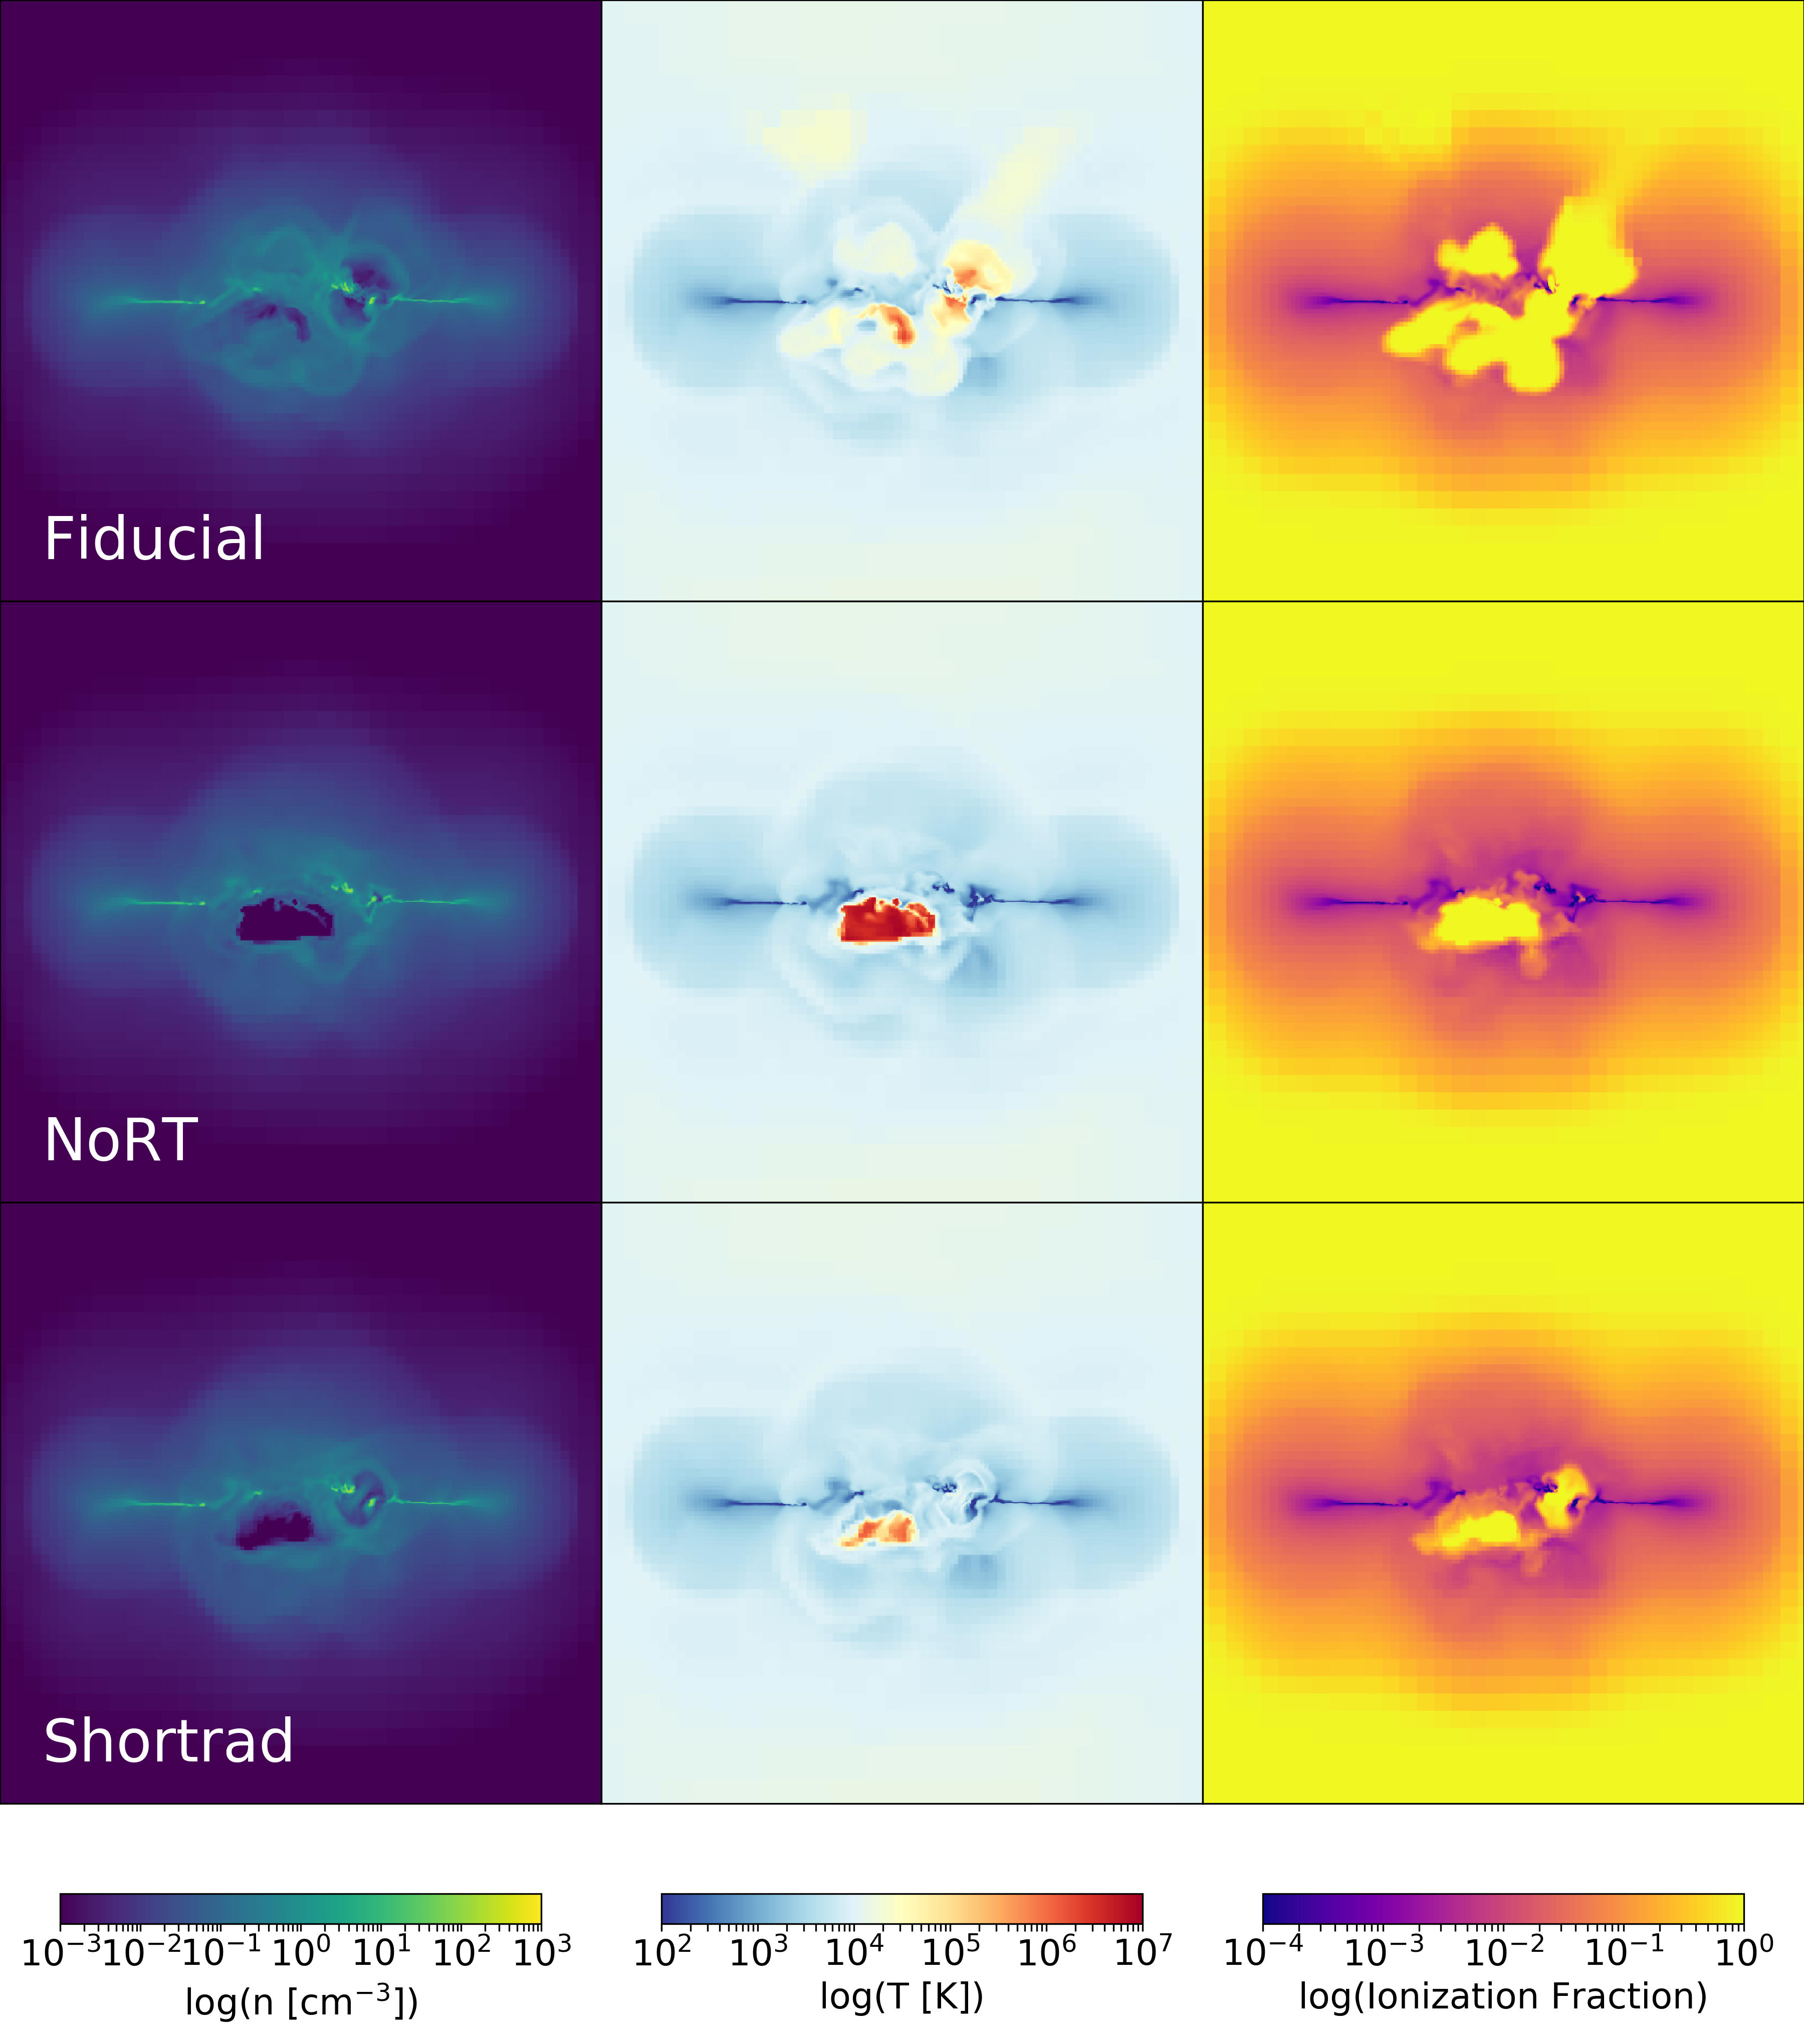
\includegraphics[width=0.99\linewidth]{DD0136_fiducial_shortrad_nort}
\caption{\textbf{In the final version of this figure I will add labels for each row marking the simulation, and a line giving the scale of each figure.}}
\label{fig:pane1l}
\end{figure*}

As these simulations evolve, the existence of these diffuse, ionized channels in the fiducial run easily allow significant outflows from SNe to escape the disk and move well into the halo of our galaxy. In contrast, the same SNe in the other two simulations are well contained, surrounded by shells of denser, neutral gas and unable to driving significant mass loss from the galaxy. In the noRT case, outflow does eventually develop, but it takes the factor of 5 increase in SFR for SN gas to finally break out from the neutral gas surrounding the galaxy.

\begin{figure*}
\centering
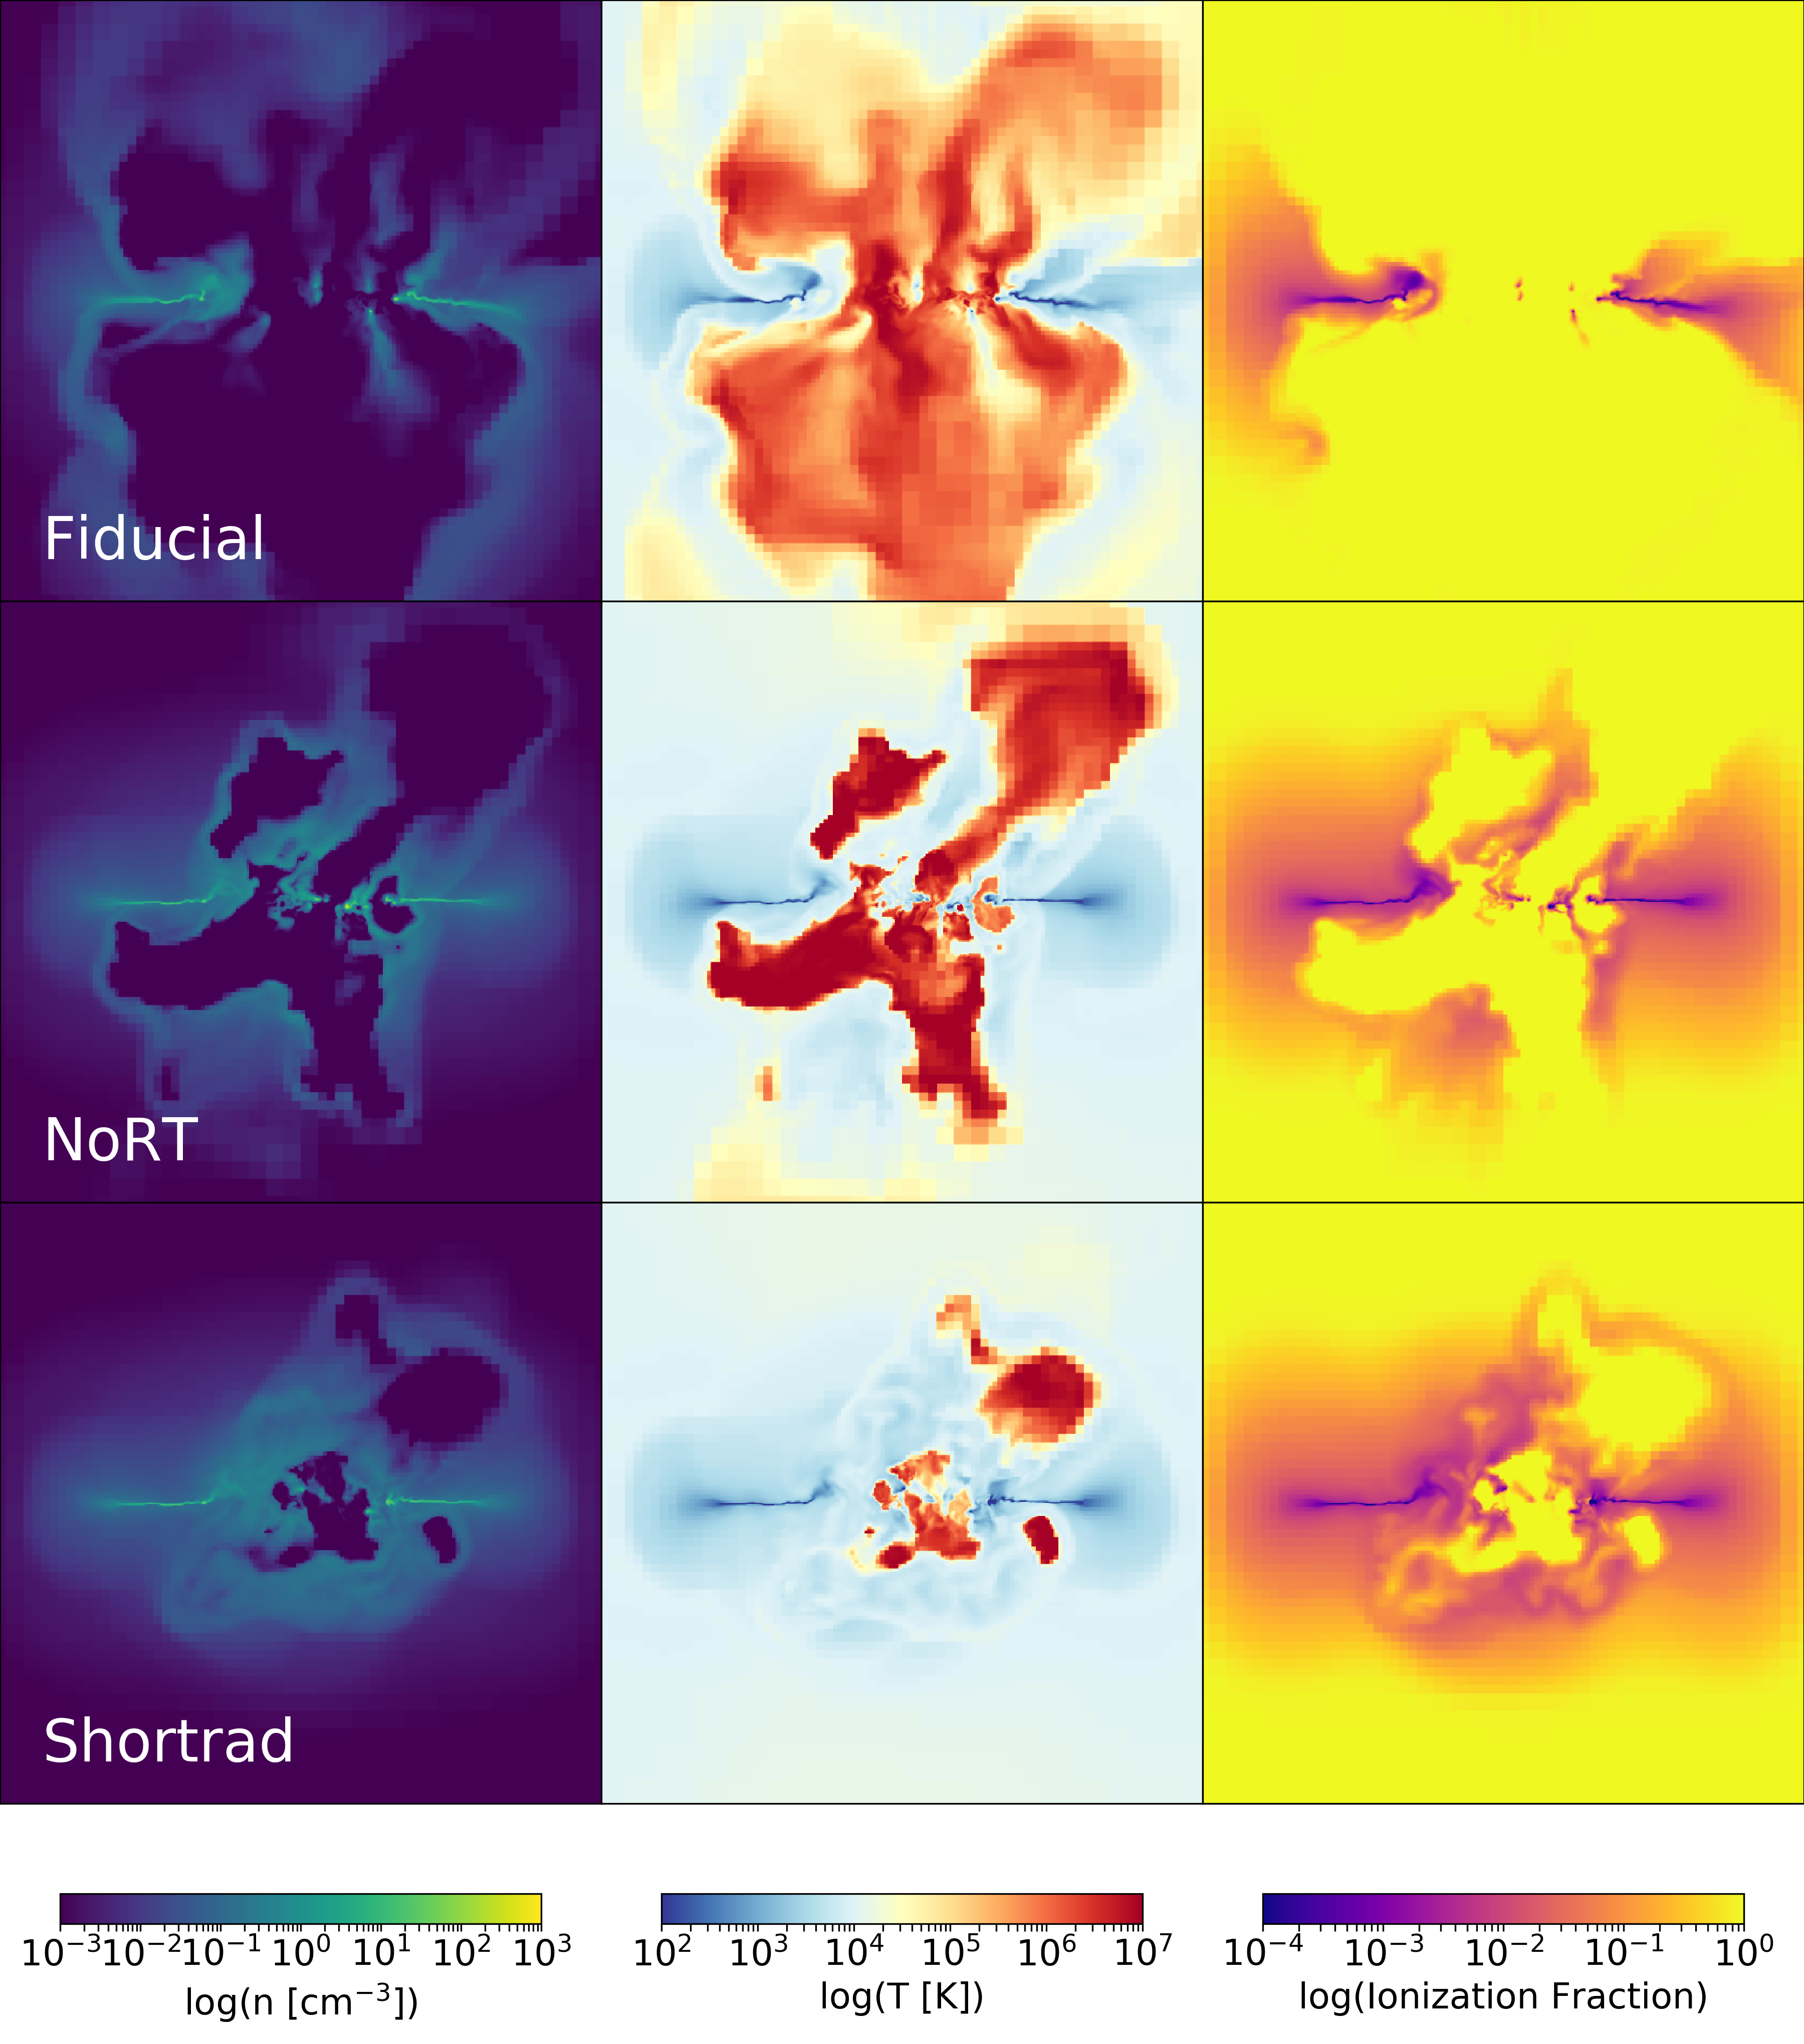
\includegraphics[width=0.99\linewidth]{DD0160_fiducial_shortrad_nort}
\caption{Panel}
\label{fig:pane2}
\end{figure*}

\section{Conclusion}  \label{sec:conclusion}
Very short. Just re-iterate points

\begin{thebibliography}{}


\end{thebibliography}

%% This command is needed to show the entire author+affilation list when
%% the collaboration and author truncation commands are used.  It has to
%% go at the end of the manuscript.
%\allauthors

%% Include this line if you are using the \added, \replaced, \deleted
%% commands to see a summary list of all changes at the end of the article.
%\listofchanges

\end{document}

% End of file `sample62.tex'.
